\documentclass[PMO,authoryear,toc,lsstdraft]{lsstdoc}
% lsstdoc documentation: https://lsst-texmf.lsst.io/lsstdoc.html
\input{meta}

% Package imports go here.
  
% Local commands go here.

%If you want glossaries
%\input{aglossary.tex}
%\makeglossaries

\title{Internet Edge Firewall Design}

% Optional subtitle
% \setDocSubtitle{A subtitle}

\author{%
Julio Constanzo
}

\setDocRef{ITTN-049}
\setDocUpstreamLocation{\url{https://github.com/lsst-it/ittn-049}}

\date{\today}

% Optional: name of the document's curator
% \setDocCurator{The Curator of this Document}

\setDocAbstract{%
This document describe the internet edge firewall design, actual setup migration and integration with Rubin's monitoring system.
}

% Change history defined here.
% Order: oldest first.
% Fields: VERSION, DATE, DESCRIPTION, OWNER NAME.
% See LPM-51 for version number policy.
\setDocChangeRecord{%
  \addtohist{1}{2021-08-18}{Unreleased}{Julio Constanzo}
  
}


\begin{document}

% Create the title page.
\maketitle
% Frequently for a technote we do not want a title page  uncomment this to remove the title page and changelog.
% use \mkshorttitle to remove the extra pages

% ADD CONTENT HERE
% You can also use the \input command to include several content files.
\section{Scope}
The scope of this document will concentrate on the hardware and software descriptions of the pfsense solution, alongside the proposed network design and integration into Rubin's network architecture. Be in mind that this document will also show images and information related to the "FY21 network re-design", so be aware that this firewall design is also part of that big picture. Migration will be also included but will not describe each activity in detail, since detailed information will be concentrated into JIRA tickets. 
\section{Hardware Description}

\subsection{Minimum hardware requirements}
The minimum hardware requirements for pfsense® 2.5.2-RELEASE on hardware not sold by Netgate are:


\begin{itemize}
    \item 64-bit amd64 (x86-64) compatible CPU
    \item 1GB or more RAM
    \item 8 GB or larger disk drive (SSD, HDD, etc)
    \item One or more compatible network interface cards
    \item Bootable USB drive or high capacity optical drive (DVD or BD) for initial installation
\end{itemize}

\subsection{Hardware to be used}
The two boxes that we will be using have the following specifications: 


\begin{table}[h]
    \begin{center}
    \begin{tabular}{ | m{5cm} | m{12cm} | }
    \hline CPU & Intel Xeon-DE D-1541 2.1 GHz FCBGA 1667 supported SoC \\ \hline
    CPU Cores & Eight Cores, 45W \\ \hline
    Networking & 
    \begin{description} 
        \item Dual LAN via Intel i350-AM2 1 Gigabit Ethernet
        \item Dual LAN via SoC 10GBase-T
        \item Virtual Machine Device Queues reduce I/O overhead
        \item Supports 10GBASE-T, 100BASE-TX, and 1000BASE-T, RJ45 output
        \item 1x Realtek RTL8201N PHY (dedicated IPMI) \end{description} \\ \hline
    Storage & 132 GB Micron M.2 SSD \\ \hline
    Memory & 16 GB DDR4 UDIMM \\ \hline
    \end{tabular}
    \end{center}
\end{table} 

\newpage

\begin{table}
    \begin{center}
    \begin{tabular}{ | m{5cm} | m{12cm} | }
    \hline Expansion &
    \begin{description} 
        \item 1x PCI-E 3.0 x 16 (in x4) AOC Slot
        \item 6x SATA3 ports \end{description} \\ \hline
    Other Ports &
    \begin{description} 
        \item 1x BMC integrated ASPEED AST2400
        \item 1x IPMI Port 
        \item 1x VGA Port
        \item 1x Fast UART 16550 Serial Port (header) \end{description} \\ \hline
    USB Ports & 2x USB 3.0 ports \\ \hline
    LED &
    \begin{description}
        \item Power LED
        \item Hard drive activity LED
        \item 2x Network activity LEDs
        \item System Overheat LED
        \item Information LED (temp., status) \end{description} \\ \hline
    Enclosure & 19" 1U Rack Mount - CSE-505-203B \\ \hline
    Form Factor & 1U 1.7"x17.2"x9.8" \\ \hline
    Cooling & 200W Low-noise PS with PFC: Active CPU fan, 40mm chassis fan \\ \hline
    Power & 
    \begin{description}
        \item 1x SATA DOM power connector
        \item 100-240V, 50-60Hz, 2.6 Amp MAX
        \item AC Inlet: IEC320-C14 (3 PIN)
        \item Power Cord: NEMA 5-15P to IEC320-Cxx \end{description} \\ \hline   
    Environmental & 
    \begin{description}
        \item 10°C to 35°C Operating Temp
        \item 8\% to 90\% Operating Relative Humidity (non-condensing) \end{description} \\ \hline
    Power Consumption & TBD W (idle) \\ \hline
    Certifications & FCC, CE, RoHS, UL \\ \hline
    \end{tabular}
    \end{center}
\end{table} 






\section{Software Description}

pfsense Plus software is a powerful firewall, router, and VPN solution that leverages a number of highly-regarded open-source projects. The software competes effectively with far more expensive, commercial alternatives and is used by hundreds of thousands of businesses, educational institutions, and government agencies all over the world. Leading secure-networking features and capabilities include:

\begin{itemize}
    \item Ad blocker (pfBlockerNG)
    \item Captive Portal
    \item CARP / HA
    \item DNS Server
    \item DHCP Server
    \item HTTP transparent / web / reverse proxy (Squid)
    \item IP / Country block list (pfBlocker)
    \item IDS/IPS
    \item Packet capture / inspection
    \item Port forwarding
    \item QOS / rate limiters
    \item Software load balancer (HA Proxy)
    \item Traffic monitoring
    \item Traffic logging, statistics, and graphs
    \item Traffic shaping
    \item VLAN
    \item Wake-on-LAN
    \item Website blocker (pfBlocker)
\end{itemize}

\subsection{Key features}

\subsubsection{Low total cost of ownership}

\begin{itemize}
    \item No artificial limits or add-ons are required to make your system fully functional.
    \item No additional usage or feature-based pricing. Enjoy unlimited users, unlimited firewall rules, unlimited IPsec tunnels, dual WAN, etc.
    \item Standard configuration with 16GB of RAM and 256GB Micron M.2 SSD*.
    \item Low power requirements to help save you money.
    \item This system is designed for a long deployment lifetime.
\end{itemize}

\subsubsection{Growth}

\begin{itemize}
    \item From firewall to Unified Threat Management, get all the security features you need to protect your home or business.
    \item Flexible configuration and support for multi-WAN, high availability, VPN, load balancing, reporting, and monitoring, etc.
    \item Add optional packages such as Snort or Suricata for IDS/IPS and network security monitoring, Squid for optimized content delivery, and SquidGuard for \item anti-spam/anti-phishing and URL filtering. 1 
    \item Maximum Active Connections: 16,000,000 (32,000,000 with 32 GB RAM)
\end{itemize}

\subsubsection{GUI Management}

\begin{itemize}
    \item Manage pfsense Plus software settings through our web-based GUI.
    \item No fumbling with a command-line interface or typing arcane commands.
\end{itemize}

\subsubsection{Secure Remote Access}

\begin{itemize}
    \item Connect via encrypted Virtual Private Networks (VPN) between your offices, let mobile workers connect securely, or connect to the Cloud.
    \item Use the built-in Amazon VPC Wizard to easily establish VPN connections with your Amazon EC2 cloud.
\end{itemize}

\subsubsection{Best For}

\begin{itemize}
    \item Medium to Large Sized Networks with 1U rack mount cabinets
    \item Medium to Large Sized Branch Office with heavy loads
    \item Managed Service Providers (MSP) / Managed Security Service Provider (MSSP) On-Premises Appliance
    \item Enterprise
    \item Anyone with High-Speed 10 Gigabit and/or 1 Gigabit Connections 
    \item Anyone with many VPN Connections
    \item Anyone with high-speed connections who wish to configure IDS/IPS features
\end{itemize}



\section{Network Design}

As explained in the scope of this document, the following network design is also related and tied to the FY21 network re-design which is also under development.

\begin{figure}
    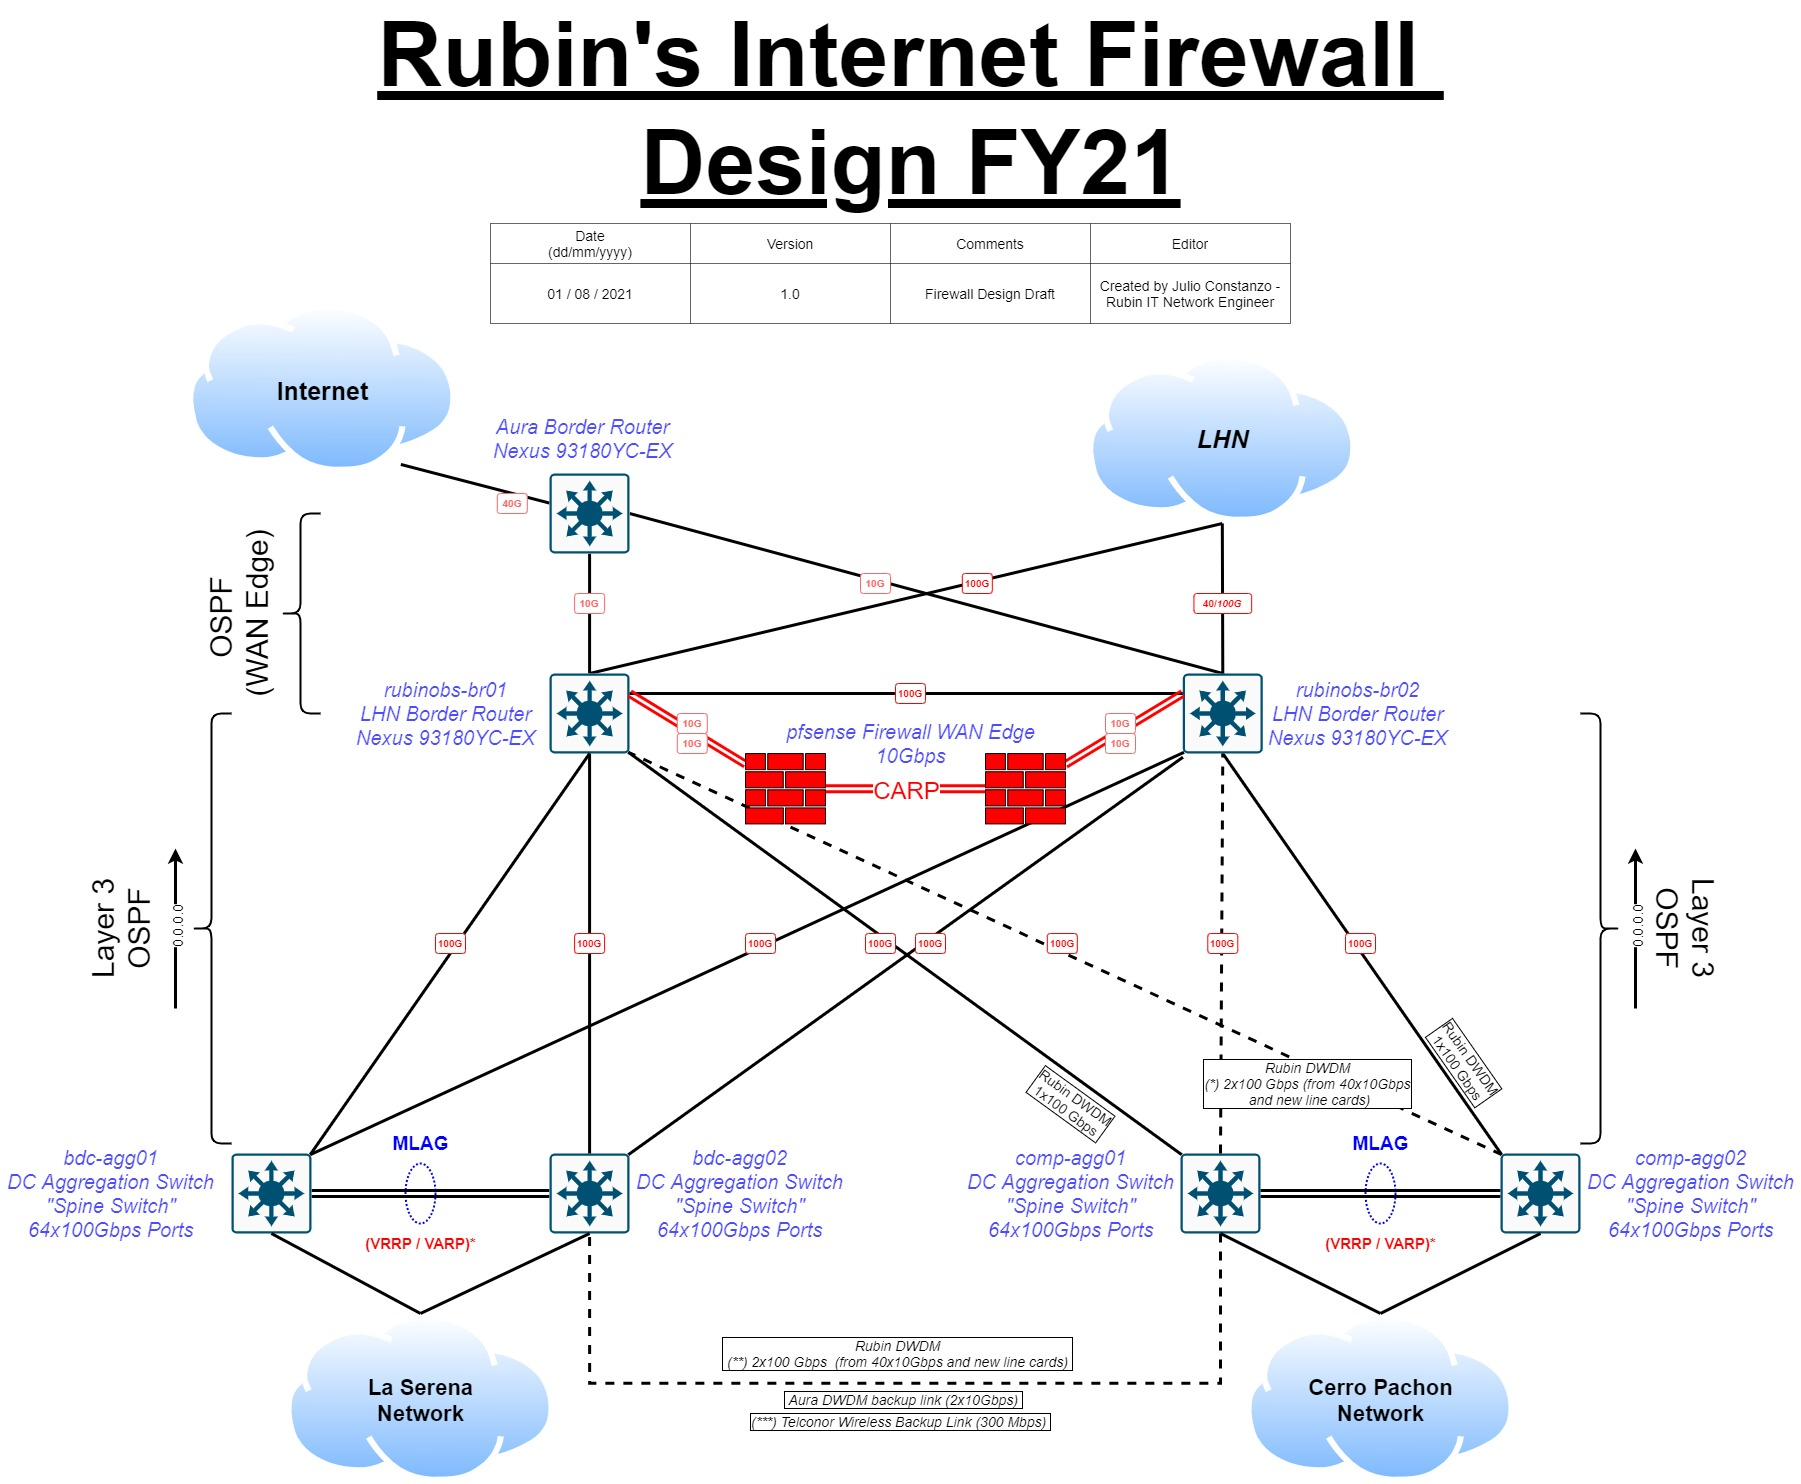
\includegraphics[width=\linewidth]{images/fw_design.jpg}
    \centering
    \caption{Internet Edge Firewall Network Design}
  \end{figure}
\section{Migration}

The two Super Micro XG-1541 chassis were already racked and mounted inside our base data center during the beginning of 2021, and are running the latest and most updated version of pfsense (2.5.2-RELEASE built on Fri Jul 02 15:33:00 EDT 2021). The two boxes have a clean installation and can be moved at will since they are inside a development environment directly connected to AURA border router for WAN access. Meanwhile, out-of-band access is made through BMC interfaces.

\subsection{Location inside Data Center}

If physical movement is required, the two boxes will be moved to rack A4 near Rubin's and AURA border routers. 10Gbps interfaces are using LC multimode fiber and FS SFP+ modules. Gigabit ethernet connections are using CAT6/CAT6a cables. Their actual location is on rack B9.

\subsection{Firewall Configurations}

pfsense has a "backup and restore" wizard which is pretty useful since also has the ability to perform area backups, meaning that can export and import specific code from/into the configuration file. Be aware that not all features are listed on the "backup area" list. Meanwhile, the "restore area" has a bigger option list.

Bear in mind that the actual 1Gbps firewall installed and in use in La Serena will be decommissioned once the new setup enters production. All configurations will be saved and used for the new 10Gbps firewall setup.

\subsection{Authentication}

Authentication will be made through IPA services. IT administrators should not use a local account unless explicitly is required (i.e during an IPA outage). The local account is only for the mandatory admin user and IT admin user. AD account only if needed.

\subsection{Interfaces}

Interfaces will require to be modified since the WAN and LAN connections will change. This will not affect CARP or BMC interfaces.

\subsection{Firewall Aliases}

Firewall Aliases can be exported and copy directly into new boxes. Aliases can be " only-restore" on pfsense web-based GUI wizard. 

\subsection{NAT Rules}

NAT rules will require to be modified since the WAN and LAN interfaces will change. NAT rules can be "backup and restore" on pfsense web-based GUI wizard.

\subsection{Firewall Rules}

Firewall rules will require to be modified since the WAN and LAN interfaces will change. Firewall rules can be "backup and restore" on pfsense web-based GUI wizard.

\subsection{CARP}

CARP interfaces are belonging to a private range that is not in use in another segment of the network which made high availability possible, so no action is required.

\subsection{Routing}

Static routes will require to be modified since the WAN and LAN interfaces will change. Static rules can be "backup and restore" on pfsense web-based GUI wizard.

\subsection{IPSec}

IPSec will require to be modified since the WAN and LAN interfaces will change. This activity will require coordination with Steward and Rubin's Tucson IT departments. IPSec can be "backup and restore" on pfsense web-based GUI wizard.

Note: Policy-Based or VTI modes are available. See availability on end-points for both solutions.

\subsection{OpenVPN}

OpenVPN will require to be modified since the WAN and LAN interfaces will change, alongside the certificates. OpenVPN configuration can be "backup and restore" on pfsense web-based GUI wizard.

Note: WireGuard has been removed from the base system in releases after pfSense Plus 21.02-p1 and pfSense CE 2.5.0 when it was removed from FreeBSD. If upgrading from a version that has WireGuard active, the upgrade will abort until all WireGuard tunnels are removed. WireGuard is available as an experimental add-on package on pfSense Plus 21.05, pfSense CE 2.5.2, and later versions. The settings for the WireGuard add-on package are not compatible with the older base system configuration.

\subsection{Snort}

Snort policies will require to be carefully applied to the correct interfaces using the correct "Pass-Lists" and "Aliases". Snort rules can NOT be "backup and restore" on pfsense web-based GUI wizard, is preferred to do it manually and proceed with caution since it's going to block Interface traffic if it's not correctly applied.
\section{Integration}

\subsection{Integration with Rubin Observatory network}

Both boxes have the possibility to be monitored by IT monitoring services such as:

\begin{itemize}
    \item Graylog: Syslog monitoring system
    \item Icinga: Heartbeat and services monitoring system
    \item Grafana: Graphic telemetry monitoring system
\end{itemize}

Note: The actual setup is integrated with Graylog and Icinga monitoring services. Grafana hasn't been used in the past, but it's good to have in our monitoring system.


\subsection{Integration with third-party services}

There is coordination to be made and emails to be sent in order to inform third-party services about our firewall changes, in order to avoid cloud or third-party services outages.
\section{Conclusion}

This firewall proposal is based on the well-known pfsense solution that is already in use on the Vera C. Rubin Observatory network, but with the benefits of 10Gbps interfaces for WAN and LAN, alongside a more well-suitable network design for base and summit facilities.

There are no hardware or software costs involved since all the materials were already under the control of the IT La Serena department, and the software is open-source based.

The activities required to perform a successful migration are less complicated than if we decided to go with another firewall solution different from pfsense. Also notice that the two new boxes are already running the latest software and are under development which is a plus in time, cost, and planning.

Again, be aware that this design is very tied to the FY21 network re-design, so most of the actual routing will change in the future to accommodate the design explained in this document, mainly on how both sites are going to reach Internet access. 


\appendix
% Include all the relevant bib files.
% https://lsst-texmf.lsst.io/lsstdoc.html#bibliographies
\section{References} \label{sec:bib}
\renewcommand{\refname}{} % Suppress default Bibliography section
\bibliography{local,lsst,lsst-dm,refs_ads,refs,books}

% Make sure lsst-texmf/bin/generateAcronyms.py is in your path
\section{Acronyms} \label{sec:acronyms}
\addtocounter{table}{-1}
\begin{longtable}{p{0.145\textwidth}p{0.8\textwidth}}\hline
\textbf{Acronym} & \textbf{Description}  \\\hline

AC & Alternating Current \\\hline
AD & Associate Director \\\hline
AOC &  AURA Oversight Council \\\hline
AURA & Association of Universities for Research in Astronomy \\\hline
CE & Communications Engagement \\\hline
CPU & Central Processing Unit \\\hline
DE & dark energy \\\hline
DNS & Domain Name Service \\\hline
DOM & Document Object Model \\\hline
FS & File System \\\hline
FY21 & Financial Year 21 \\\hline
GB & Gigabyte \\\hline
GUI & Graphical User Interface \\\hline
HDD &  Hard Disk Drive \\\hline
HTTP & HyperText Transfer Protocol \\\hline
IP & Internet Protocol \\\hline
IPS & Integrated Project Schedule \\\hline
IPsec & Internet Protocol Security \\\hline
IT & Information Technology \\\hline
LAN & Local Area Network \\\hline
LED & Light-Emitting Diode \\\hline
NAT & Network Address Translation \\\hline
PCI & Peripheral Component Interconnect \\\hline
PMO & Project Management Office \\\hline
PS & Project Scientist \\\hline
RAM & Random Access Memory \\\hline
SATA & Serial Advanced Technology Attachment \\\hline
SSD & Solid-State Disk \\\hline
TBD & To Be Defined (Determined) \\\hline
URL & Universal Resource Locator \\\hline
USB & Universal Serial Bus \\\hline
VLAN &  Virtual Local Area Network \\\hline
VPC &  Virtual Private Cloud \\\hline
VPN & virtual private network \\\hline
WAN & Wide Area Network \\\hline
\end{longtable}

% If you want glossary uncomment below -- comment out the two lines above
%\printglossaries





\end{document}
